\documentclass{webofc}
\usepackage[varg]{txfonts}
\usepackage{graphicx}
\usepackage{minted}

% 6 pages excluding references!

\begin{document}
\title{Awkward Arrays in Python, C++, and Numba}

\author{%
\firstname{Jim} \lastname{Pivarski}\inst{1}\fnsep\thanks{\email{pivarski@princeton.edu}} \and
\firstname{Peter} \lastname{Elmer}\inst{1}\fnsep\thanks{\email{Peter.Elmer@cern.ch}} \and
\firstname{David} \lastname{Lange}\inst{1}\fnsep\thanks{\email{David.Lange@cern.ch}}}

\institute{Princeton University}

\abstract{%
  Insert your english abstract here.
}

\maketitle

\section{Introduction}

Columnar data structures, in which identically typed data fields are contiguous in memory, are a good fit to physics analysis use-cases. This was recognized as early as 1989 when column-wise ntuples were added to PAW and in 1995 when ``splitting'' was added to the ROOT file format. In the past decade, with the Google Dremel paper [ref], the Parquet file format [ref], the Arrow memory interchange format [ref], and the inclusion of ``ragged tensors'' in TensorFlow [ref], the significance of hierarchical columnar data structures has been recognized beyond particle physics.

With the exception of the Columnar Objects experiment of T.\ Mattis et.\ al.\ [ref] and the XND library [ref], all of these projects focus on representing, storing, and transmitting columnar data structures, rather than operating on them. Physicists need to apply structure-changing transformations to search for decay topology candidates and other tasks that can change the level of nesting and multiplicity of their data. Operations of this complexity can be defined as a suite of primitives, allowing for NumPy-like convenience in Python \mbox{[2018 CHEP ref].\hspace{-1 cm}}

The Awkward Array library [2018 ROOT workshop ref] was created to provide these operations on arrays that are easily convertible to the other libraries (zero-copy in some cases). Since its release in September 2018, it has become one of the most widely pip-installed packages for particle physics (see Figure~\ref{fig:pip-timeline}).

\begin{figure}
\begin{center}
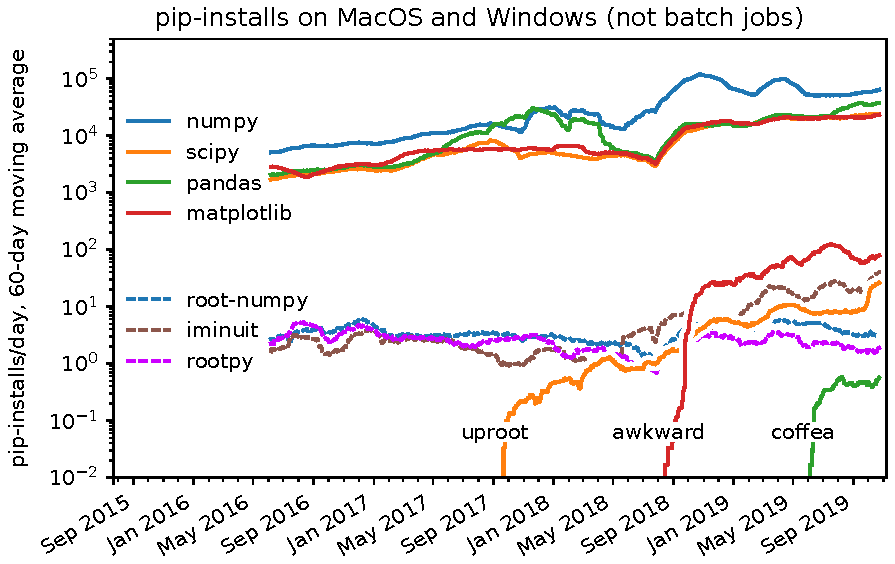
\includegraphics[width=0.75\linewidth]{pip-timeline.pdf}
\end{center}
\caption{Number of pip-installations per day (smoothed by a 60-day moving average) for popular data analysis libraries (numpy, scipy, pandas, matplotlib) and particle physics libraries (root-numpy, iminuit, rootpy, uproot, awkward, coffea) on operating systems not used for batch jobs (MacOS and Windows). \label{fig:pip-timeline}}
\end{figure}

Feedback from physicists, such as the interviews we reported previously [2019 ACAT paper ref] and in private conversations at a series of tutorials, has revealed that physicists appreciate the NumPy-like interface when it's easy to see how an analysis task can be expressed that way, but still need an interface for imperative programming. Some names were poorly chosen, leading to confusion and name-conflicts, and more of the library's internal structure should be hidden from end-users. In addition, the original library's pure NumPy implementation has been hard to extend and maintain.

All of these issues argue for a redesign of the library, keeping the core concepts that work, restructuring the internals for maintainance, and presenting a simpler, more uniform user interface. The Awkward Array reimplementation project has been dubbed ``Awkward 1.0'' and has been allocated as a 6-month task from September 2019 to March 2020.

\section{Architecture}

\subsection{High-level Python layer}

\subsection{C++ layer}

\subsection{Numba layer}

\subsection{Kernels layer}

\section{Record-oriented $\to$ columnar}

% \subsection{Deeply nested data from ROOT}

\section{Status}

\section{Conclusion}




%% \section{Introduction}
%% \label{intro}
%% Your text comes here. Separate text sections with

%% \section{Section title}
%% \label{sec-1}
%% For bibliography use \cite{RefJ}

%% % BibTeX or Biber users please use (the style is already called in the class, ensure that the "woc.bst" style is in your local directory)
%% % \bibliography{name or your bibliography database}
%% %
%% % Non-BibTeX users please use
%% \begin{thebibliography}{}
%% % and use \bibitem to create references.
%% \bibitem{RefJ}
%% Journal Author, Journal \textbf{Volume}, page numbers (year)
%% \end{thebibliography}

\end{document}
